\chapter{Einleitung}
\section{Eins - Eins}
\subsection{Eins - Eins - Eins}

% Die Logos sind veraltet und duerfen zurzeit nicht verwendet werden!
% Auf Seite \pageref{Logo} in Abbildung \ref{Logo} befindet sich das SE Logo.

Absätze werden in Latex durch eine Leerzeile voneinder getrennt. Die Grundlagen zur UML/P finden sich in \cite{Rum11}

Anstatt die Absätze durch einen größeren Abstand voneinander zu trennen, kann man auch die erste Zeile einrücken.

Eine Website zitiert man so \cite{SE10} und hier gibt es MontiCore \cite{Mon10}. 

Das sieht dann z.B. so aus ...
\setlength{\parindent}{3ex}
\setlength{\parskip}{0ex}

Neuer Absatz ... Neuer Absatz ... Neuer Absatz ... Neuer Absatz ... Neuer Absatz ... Neuer Absatz ... Neuer Absatz ... Neuer Absatz ...

Neuer Absatz ... Neuer Absatz ... Neuer Absatz ... Neuer Absatz ... Neuer Absatz ... Neuer Absatz ... Neuer Absatz ... Neuer Absatz ...

Eine der beiden Varianten MUSS man wählen, welche ist jedoch egal.

\cleardoublepage

\chapter{Related work}
In this section, different tutorials will be analyzed to extract the most convenient and important features. The result will be used to increase the productivity and efficiency of the teaching process. Different tutorials have been taken into consideration from various domains: programming languages, numerical computing environment and so on. The main goal is to find the most useful features and integrate them.

In the section 3.1 will be introduced very powerful tool which is used in different areas for building systems with 
any complexity level.

\section{Simulink}
Simulink has been created by Mathworks(link). Simulink is a block diagram environment for various domain simulation and Model-Based Design. It also involves C\&C models into the modeling process. Users create models in a visual way, not writing the code. You can see an example of a fuel calculation subsystem(see figure \ref{fig:simulink}). There are depicted the incoming and outgoing ports of the schema, like est\_airflow or fuel\_rate. And the connections between the components inside. The schema is very useful for visual perception, you can easily see connections between elements and understand the logic behind that. If you had just textual representation of the elements and connections between, it would de much harder to imagine the whole schema and i.e. find some issue with an accidentally connected port or disconnected one.

\begin{figure}[h!]
    \centering
    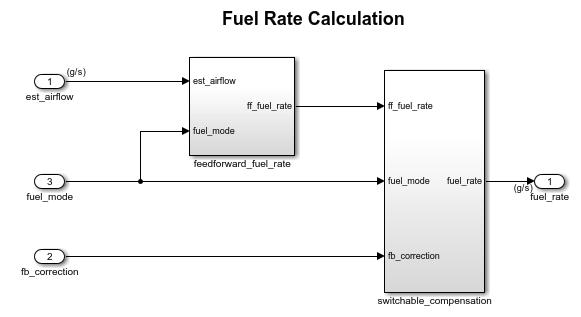
\includegraphics[width=0.7\linewidth]{src/pic/simulink}
    \caption{Simulink schema example.}
    \label{fig:simulink}
\end{figure}

Simulink has plenty of tutorials in many different areas with detailed description and videos on solving it which describes it step-by-step. It is very helpful to have step-by-step solution with detailed description for understanding all important details. Because on this understanding of essentials, is build the future knowledge and depends future success. But there is some weakness in an education process. The issue is, that they don't have methods for validating the correctness of the user's solution and does not encourage the users to try it out by themselves, just copy the sample solution.

\section{Rust}
Rust(Link) is a very popular programming language the prevalence of which is growing every day. It has a consistent tutorial which describes language constructs with gradually increasing complexity. It has the informative and structured index, where users can easily jump from one topic to another almost instantly and then just go back to the place where he was reading before. They use highlighted ares to show some code examples, which facilitate understanding of presented materials. It is possible to copy some parts of the code and even directly execute it in a browser(see figure \ref{fig:rust}).

\begin{figure}[h!]
    \centering
    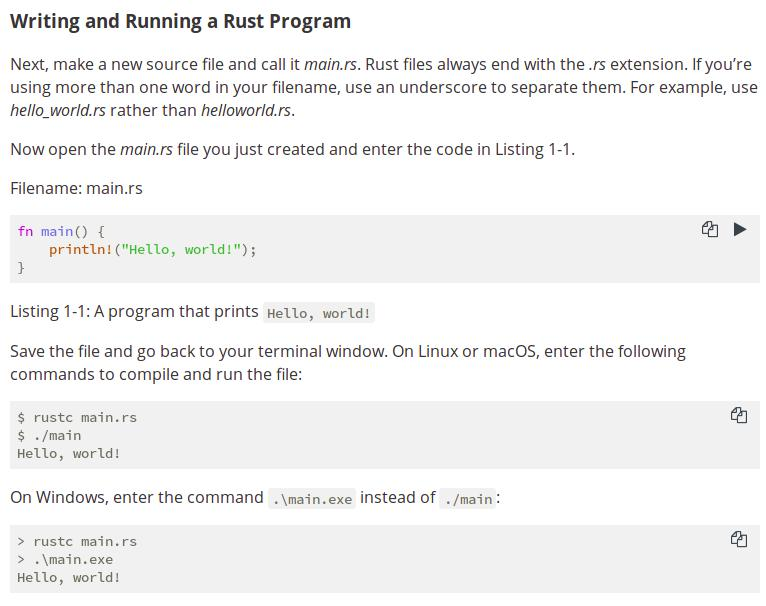
\includegraphics[width=0.7\linewidth]{src/pic/rust}
    \caption{Rust tutorial example.}
    \label{fig:rust}
\end{figure}

To execute the given code, you just have to click on the play button in the upper right corner and in several second the result will be displayed. This is very important and useful feature, because students can directly see what the code does. At the given example it is pretty straightforward, but if you have some computation, not even complex one, it is already not so easy to imagine the output.
Nevertheless, even in this short example, there is some issues related to the compilation process. Namely, the different compilation and execution process for diverse platforms(Windows, Linux, macOS). It means, that we have to install the compiler to use it during the learning process. It would be very convenient to have all these features directly in the web-browser, without installation.

\section{Microsoft Z3 Solver}
Z3 is a state-of-the art theorem prover from Microsoft(link). It provides similar experience compare to Rust tutorial but with some improvements, which simplify the studying process. There is a possibility, not only to execute the given code from the current example directly in the browser, but edit the code, and still see the result almost instantly due to in-browser execution. It helps to see the direct binding between written commands and the real result, that improves understanding of given material.

\begin{figure}[h!]
    \centering
    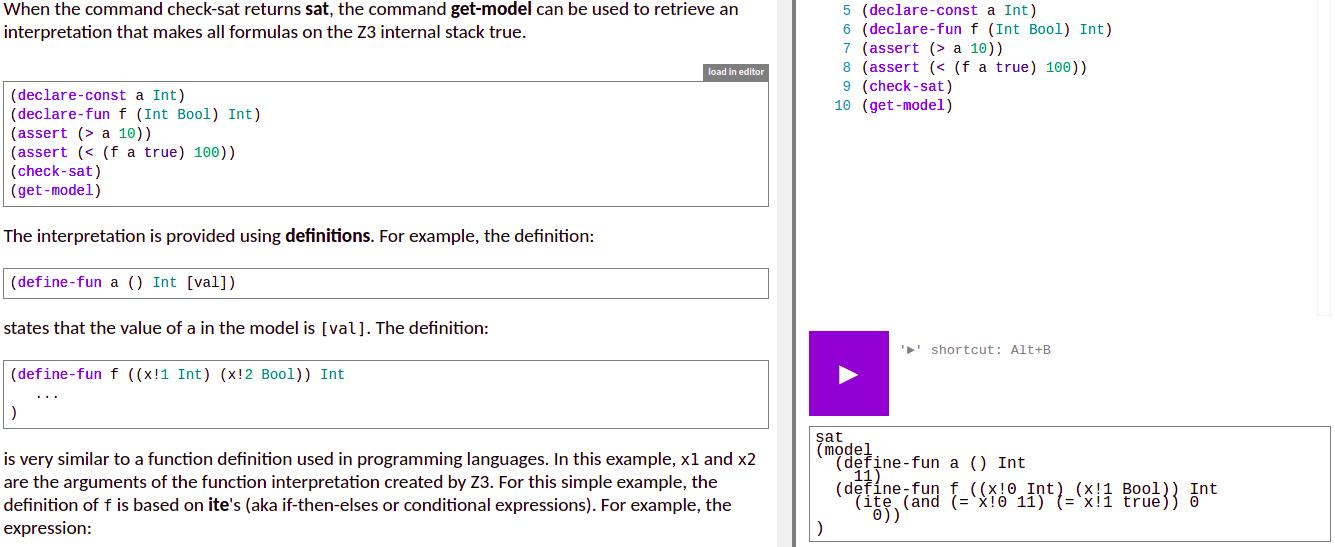
\includegraphics[width=\linewidth]{src/pic/z3}
    \caption{Z3 tutorial example.}
    \label{fig:z3}
\end{figure}

In the figure \ref{fig:z3}, you can see the code given in a tutorial on the left hand side. On the right hand side, there is the code which has been executed and the result appeared below. Then you can adjust the code to check some hypothesis, and instantly see the result. By doing this, students can check their understanding of an explained material.
Another advantage in this tutorial is a in-browser execution. Students do not have to install anything and can directly work in browsers. It means, the operating system(OS) does not have any influence on the execution and compilation process. Any OS can be used, it is necessary to have a web-browser. If this tutorial will be used directly on a lecture, then students just enter the URL in a browser and can instantly try to execute some examples.

\section{Octave Online}
Octave Online(link) is web-playground fot a high-level language Octave, which is primarily intended for numerical computations. It has a simple and intuitive interface despite the complexity of the internal implementation. It provides directly in a browser fast execution with errors handling. Even if you do complex computations it is not needed to install any software on the PC. Everything works out of the box.


\cleardoublepage